\chapter{Supplemental Material}

\begin{figure}[!ht]

\includegraphics[width=0.7\textwidth]{../figures/chaptersDesign.pdf}
\caption{Overview of the age class, species, provenance of the trees used in each study along with the type of study each chapter consists of. The colored lines represent the period of the growth data and the shaded areas are the phenological data. Both are colour-coded by project. Each phylogram illustrates the species used in each project. The map illustrates the four different provenances used in Chapter 1, and the star represents the study location of both chapters}
\label{fig:chaptdesign}
\end{figure}


\setlength{\tabcolsep}{3pt}
% latex table generated in R 4.5.1 by xtable 1.8-4 package
% Wed Jul 15 10:34:16 2026
\begin{table}[ht]
\centering
\caption{Provenance coordinates and count per species and provenances out of a total of 81 individual trees sampled from the United States of America (in Massachusetts (MA) and New Hampshire(NH)) and Canada (in Quebec (Qc)).} 
\label{tab:provs}
\begin{tabular}{lrrrrrr}
  \hline
Provenance & Longitude & Latitude & \textit{A. incana} & \textit{B. alleghaniensis} & \textit{B. papyrifera} & \textit{B. populifolia} \\
 & & & $(n = 29)$ & $(n = 20)$ & $(n = 7)$ & $(n = 25)$ \\
\hline
 \hline
 Harvard Forest (MA) & -72.2 & 42.5 & 7 & 0 & 4 & 7 \\ 
  White Mountains (NH) & -71.0 & 44.1 & 6 & 7 & 0 & 9 \\ 
  Dartmouth College (NH) & -70.7 & 44.9 & 8 & 7 & 2 & 9 \\ 
  St-Hippolyte (Qc) & -74.0 & 46.0 & 8 & 6 & 1 & 0 \\ 
   \hline
\end{tabular}
\end{table}


% Phenology observations time series
\begin{figure}[!ht]

\includegraphics[width=0.6\textwidth]{/Users/christophe_rouleau-desrochers/github/wildchrokie/analyses/figures/empiricalData/phenoTimeseries.pdf}
\caption{Leaf phenology monitoring frequency across years. We monitored leaf phenology once or twice per week for three years, though the frequency varied within and across years. Each histogram bin represents the number of observations that were made during a period of 14 days and the lines represent the earliest, the average and last recorded budburst observations. This demonstrates that across the different frequencies of observation, distances between early spring phenophases were similar across years.}
\label{fig:phenoTimeSeries}
\end{figure}

% Rw per year for allometry
\begin{figure}[!ht]

\includegraphics[width=1\textwidth]{/Users/christophe_rouleau-desrochers/github/wildchrokie/analyses/figures/empiricalData/rwXyearAll.pdf}
\caption{We show the potential allometry patterns across all years we had ring width for. For this, we randomly sampled 20 trees from our dataset and represent their ring width (mm) for each year.}
\label{fig:allom}
\end{figure}


%-------------------------------------------------------------------------------
% Supplemental Results
%-------------------------------------------------------------------------------
\clearpage
\subsection*{Supplemental Results} 


% latex table generated in R 4.5.1 by xtable 1.8-4 package
% Wed Jul 15 10:34:16 2026
\begin{table}[ht]
\centering
\caption{Species level slope parameters which represent ring width change (log(mm)), per adjusted predictor (see `Data analyses' in Methods for more details). We report estimates as mean and 90\% uncertainty intervals (in square brackets) across our four different phenological predictors (GDD: growing degree days, GSL: growing season length, SOS: start of season and EOS: end of season).} 
\label{tab:wc_slope_table}
\begin{tabular}{lllll}
  \hline
Species & GDD & GSL & SOS & EOS \\ 
  \hline
\textit{A. incana} & 0.02 [-0.01, 0.05] & 0.05 [0.00, 0.10] & -0.07 [-0.14, -0.01] & -0.01 [-0.07, 0.04] \\ 
  \textit{B. alleghaniensis} & 0.04 [0.00, 0.08] & 0.03 [-0.03, 0.09] & 0.10 [0.01, 0.20] & 0.12 [0.05, 0.18] \\ 
  \textit{B. papyrifera} & 0.15 [0.06, 0.23] & 0.18 [0.05, 0.32] & 0.05 [-0.11, 0.21] & 0.21 [0.09, 0.33] \\ 
  \textit{B. populifolia} & 0.07 [0.02, 0.12] & 0.06 [-0.02, 0.13] & 0.05 [-0.07, 0.16] & 0.10 [0.03, 0.17] \\ 
   \hline
\end{tabular}
\end{table}


% latex table generated in R 4.5.1 by xtable 1.8-4 package
% Wed Jul 15 10:34:16 2026
\begin{table}[ht]
\centering
\caption{The effect of provenance on ring widths (log(mm)). We report these intercept estimates as mean and 90\% uncertainty intervals (in square brackets) across our four different predictors (GDD: growing degree days, GSL: growing season length, SOS: start of season and EOS: end of season).} 
\label{tab:wc_asite_table}
\begin{tabular}{lllll}
  \hline
Provenance & GDD & GSL & SOS & EOS \\ 
  \hline
Harvard Forest (MA) & -0.10 [-0.33, 0.07] & -0.08 [-0.32, 0.09] & -0.05 [-0.25, 0.12] & -0.09 [-0.33, 0.08] \\ 
  White Mountains (NH) & 0.08 [-0.09, 0.29] & 0.08 [-0.08, 0.31] & 0.09 [-0.07, 0.30] & 0.08 [-0.09, 0.29] \\ 
  Dartmouth College (NH) & -0.03 [-0.22, 0.14] & -0.04 [-0.23, 0.14] & -0.06 [-0.26, 0.10] & -0.03 [-0.23, 0.15] \\ 
  St-Hippolyte (Qc) & 0.04 [-0.14, 0.24] & 0.04 [-0.14, 0.26] & 0.02 [-0.15, 0.22] & 0.04 [-0.14, 0.26] \\ 
   \hline
\end{tabular}
\end{table}


% latex table generated in R 4.5.1 by xtable 1.8-4 package
% Wed Jul 15 10:34:16 2026
\begin{table}[ht]
\centering
\caption{Summary output of each parameter from our four predictors, using ring width (log(mm)) as the response variable. We report estimates as mean and 90\% uncertainty intervals (in square brackets) across our four different predictors (GDD: growing degree days, GSL: growing season length, SOS: start of season and EOS: end of season). See `Data analyses' in Methods section for more details.} 
\label{tab:tab_all}
\begin{tabular}{lllll}
  \hline
Parameter & GDD & GSL & SOS & EOS \\ 
  \hline
$\alpha$ & -0.62 [-4.69, 3.53] & 0.04 [-3.90, 4.04] & 1.12 [-2.61, 4.85] & -1.33 [-5.48, 2.73] \\ 
  $\sigma_{\alpha_{treeid}}$ & 0.17 [0.05, 0.27] & 0.17 [0.05, 0.28] & 0.21 [0.11, 0.30] & 0.18 [0.06, 0.28] \\ 
  $\sigma_{\alpha_{prov}}$ & 0.17 [0.02, 0.47] & 0.17 [0.02, 0.48] & 0.17 [0.02, 0.46] & 0.18 [0.02, 0.49] \\ 
  $\sigma_{y}$ & 0.48 [0.43, 0.53] & 0.48 [0.44, 0.53] & 0.47 [0.43, 0.52] & 0.47 [0.42, 0.52] \\ 
  $\beta_{species_{A. incana}}$ & 0.02 [-0.01, 0.05] & 0.05 [0.00, 0.10] & -0.07 [-0.14, -0.01] & -0.01 [-0.07, 0.04] \\ 
  $\beta_{species_{B. alleghaniensis}}$ & 0.04 [0.00, 0.08] & 0.03 [-0.03, 0.09] & 0.10 [0.01, 0.20] & 0.12 [0.05, 0.18] \\ 
  $\beta_{species_{B. papyrifera}}$ & 0.15 [0.06, 0.23] & 0.18 [0.05, 0.32] & 0.05 [-0.11, 0.21] & 0.21 [0.09, 0.33] \\ 
  $\beta_{species_{B. populifolia}}$ & 0.07 [0.02, 0.12] & 0.06 [-0.02, 0.13] & 0.05 [-0.07, 0.16] & 0.10 [0.03, 0.17] \\ 
  $\alpha_{prov_{Dartmouth College (NH)}}$ & -0.03 [-0.22, 0.14] & -0.04 [-0.23, 0.14] & -0.06 [-0.26, 0.10] & -0.03 [-0.23, 0.15] \\ 
  $\alpha_{prov_{Harvard Forest (MA)}}$ & -0.10 [-0.33, 0.07] & -0.08 [-0.32, 0.09] & -0.05 [-0.25, 0.12] & -0.09 [-0.33, 0.08] \\ 
  $\alpha_{prov_{St-Hippolyte (Qc)}}$ & 0.04 [-0.14, 0.24] & 0.04 [-0.14, 0.26] & 0.02 [-0.15, 0.22] & 0.04 [-0.14, 0.26] \\ 
  $\alpha_{prov_{White Mountains (NH)}}$ & 0.08 [-0.09, 0.29] & 0.08 [-0.08, 0.31] & 0.09 [-0.07, 0.30] & 0.08 [-0.09, 0.29] \\ 
  $\alpha_{year_{2018}}$ & 0.19 [-0.77, 1.15] & 0.22 [-0.71, 1.19] & 0.21 [-0.73, 1.15] & 0.24 [-0.72, 1.17] \\ 
  $\alpha_{year_{2019}}$ & 0.18 [-0.79, 1.14] & 0.09 [-0.85, 1.06] & 0.11 [-0.83, 1.05] & 0.12 [-0.84, 1.06] \\ 
  $\alpha_{year_{2020}}$ & -0.43 [-1.40, 0.53] & -0.35 [-1.29, 0.61] & -0.38 [-1.32, 0.58] & -0.47 [-1.44, 0.47] \\ 
  $\alpha_{species_{A. incana}}$ & 1.06 [-3.19, 5.21] & 0.20 [-3.87, 4.27] & 1.54 [-2.12, 5.13] & 3.08 [-1.30, 7.45] \\ 
  $\alpha_{species_{B. alleghaniensis}}$ & 0.21 [-3.97, 4.34] & 0.44 [-3.65, 4.46] & -1.89 [-5.68, 1.93] & -1.81 [-6.32, 2.74] \\ 
  $\alpha_{species_{B. papyrifera}}$ & -4.00 [-8.89, 0.75] & -2.60 [-7.15, 1.93] & -0.77 [-5.06, 3.47] & -5.54 [-11.15, 0.12] \\ 
  $\alpha_{species_{B. populifolia}}$ & -0.66 [-4.94, 3.63] & 0.28 [-3.96, 4.44] & -0.48 [-4.35, 3.35] & -0.88 [-5.32, 3.75] \\ 
   \hline
\end{tabular}
\end{table}


% latex table generated in R 4.5.1 by xtable 1.8-4 package
% Wed Jul 15 10:34:16 2026
\begin{table}[ht]
\centering
\caption{Summary output of each parameter from our four predictors, using basal area increment (log($mm^2$)) as the response variable. We report estimates as mean and 90\% uncertainty intervals (in square brackets) across our four different predictors (GDD: growing degree days, GSL: growing season length, SOS: start of season and EOS: end of season). See data analyses section for more details.} 
\label{tab:BAItab}
\begin{tabular}{ll}
  \hline
Parameter & Estimate \\ 
  \hline
$\alpha$ & 0.62 [-4.52, 5.84] \\ 
  $\sigma_{\alpha_{treeid}}$ & 0.52 [0.41, 0.64] \\ 
  $\sigma_{\alpha_{prov}}$ & 0.27 [0.03, 0.73] \\ 
  $\sigma_{y}$ & 0.63 [0.57, 0.70] \\ 
  $\beta_{species_{A. incana}}$ & 0.11 [-0.03, 0.25] \\ 
  $\beta_{species_{B. alleghaniensis}}$ & 0.20 [0.02, 0.36] \\ 
  $\beta_{species_{B. papyrifera}}$ & 0.92 [0.49, 1.34] \\ 
  $\beta_{species_{B. populifolia}}$ & 0.41 [0.20, 0.61] \\ 
  $\alpha_{site_{Dartmouth College (NH)}}$ & -0.11 [-0.47, 0.17] \\ 
  $\alpha_{site_{Harvard Forest (MA)}}$ & -0.09 [-0.45, 0.19] \\ 
  $\alpha_{site_{St-Hippolyte (Qc)}}$ & 0.06 [-0.23, 0.42] \\ 
  $\alpha_{site_{White Mountains (NH)}}$ & 0.15 [-0.11, 0.52] \\ 
  $\alpha_{year_{2018}}$ & -0.36 [-1.32, 0.61] \\ 
  $\alpha_{year_{2019}}$ & 0.33 [-0.65, 1.32] \\ 
  $\alpha_{year_{2020}}$ & -0.04 [-1.01, 0.94] \\ 
  $\alpha_{species_{A. incana}}$ & 3.23 [-2.25, 8.55] \\ 
  $\alpha_{species_{B. alleghaniensis}}$ & 2.09 [-3.40, 7.54] \\ 
  $\alpha_{species_{B. papyrifera}}$ & -7.59 [-14.84, -0.29] \\ 
  $\alpha_{species_{B. populifolia}}$ & -0.07 [-5.98, 5.57] \\ 
   \hline
\end{tabular}
\end{table}


% Full vs restricted data comparison for Wildchrokie
\begin{figure}[!ht]

\includegraphics[width=1\textwidth]{../figures/wildchrokie/growthModelsMain/FullVSRestricted.pdf} 
\caption{Full vs most restricted datasets for the model with start of season (a-d) and end of season (d-h) as the predictor. Each panel represent the different parameters used to fit the models. $\sigma$ (a, e), $\alpha_{species}$ (c, g) and $\alpha_{year}$ (d,h) represent the ring width (log(mm)) for species and year, respectively. $\beta_{species}$ (b, f) represent the change in ring width (log(mm))/adjusted predictor, for each species (see 'Data analyses' section in Methods for more details).} 
\label{fig:wcSOSEOScomparison}
\end{figure}

% XY facetted by species GDD
\begin{figure}[!ht]
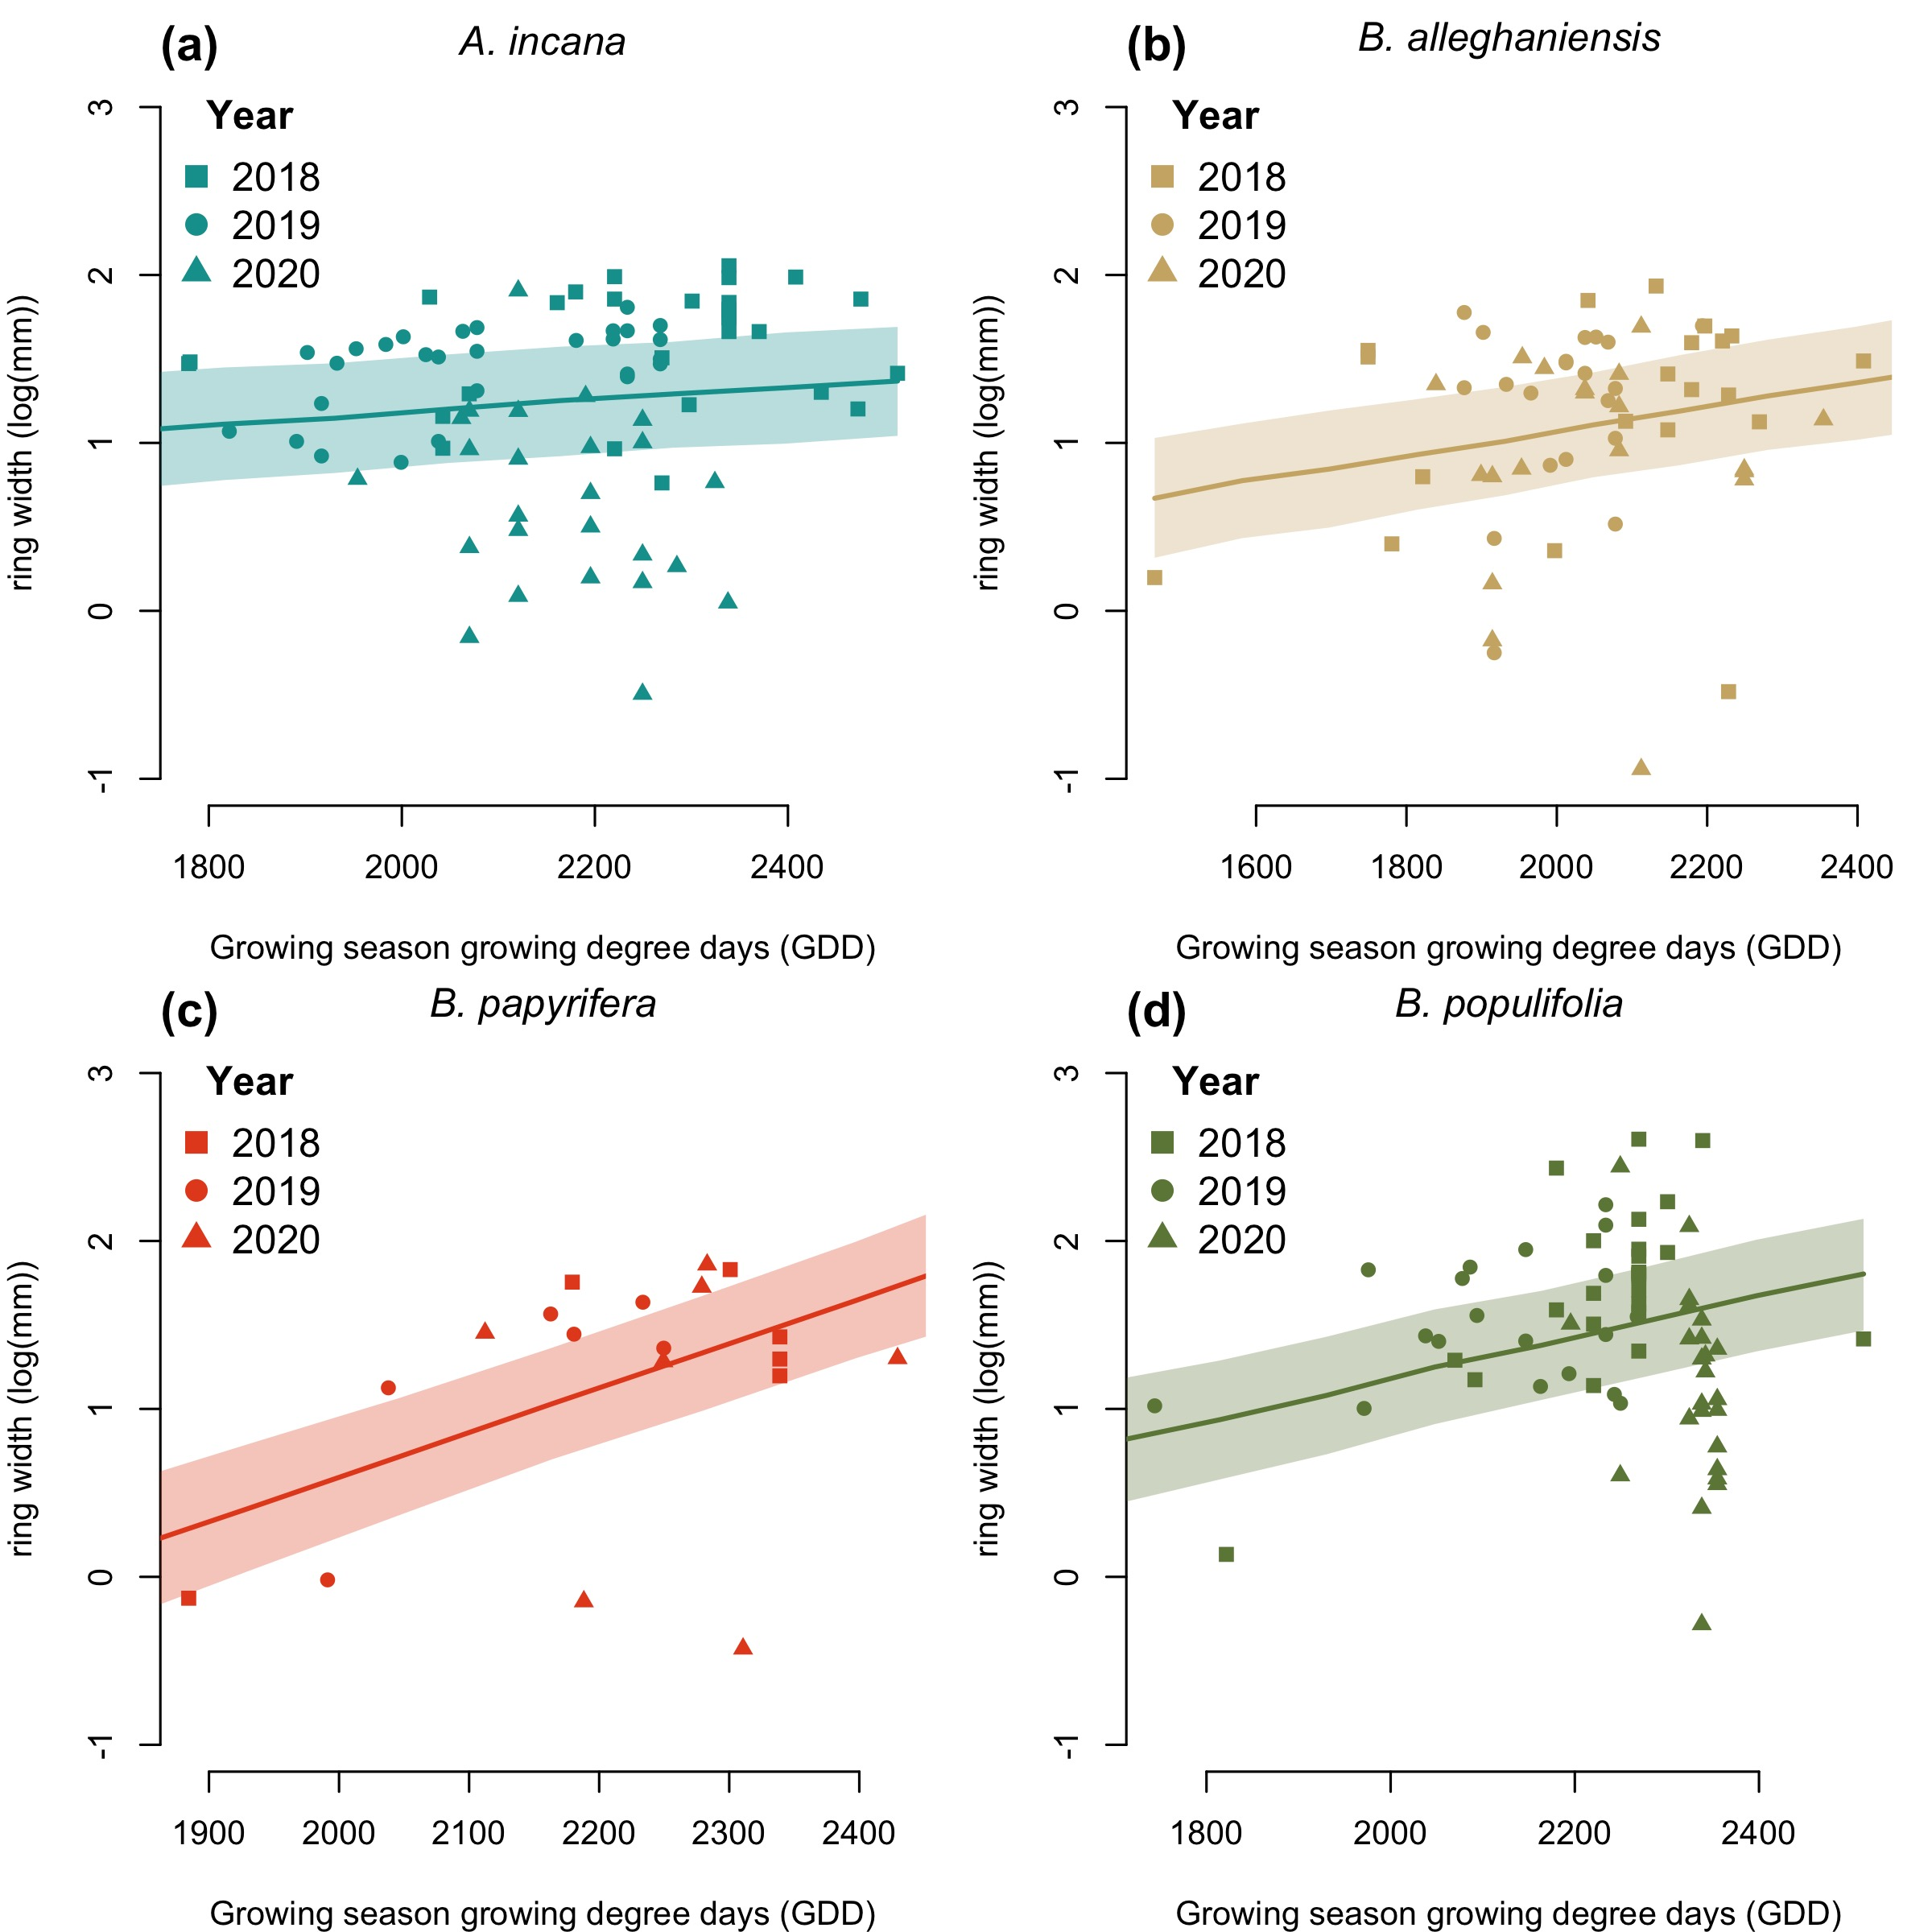
\includegraphics[width=0.8\textwidth]{../figures/wildchrokie/growthModelsMain/growthModelSlopesperSppFacet.jpeg}
\caption{Ring width (log(mm)) trends in response to thermal season (growing degree days). The plots are the reconstructed species estimates posterior distribution with error. The lines represent the mean of the posterior distribution and the shaded area, the 50\% UI at each predictor value. The dots are the empirical data shaped by year.}
\label{fig:wcxyGDD}
\end{figure}

% XY facetted by species GSL
\begin{figure}[!ht]
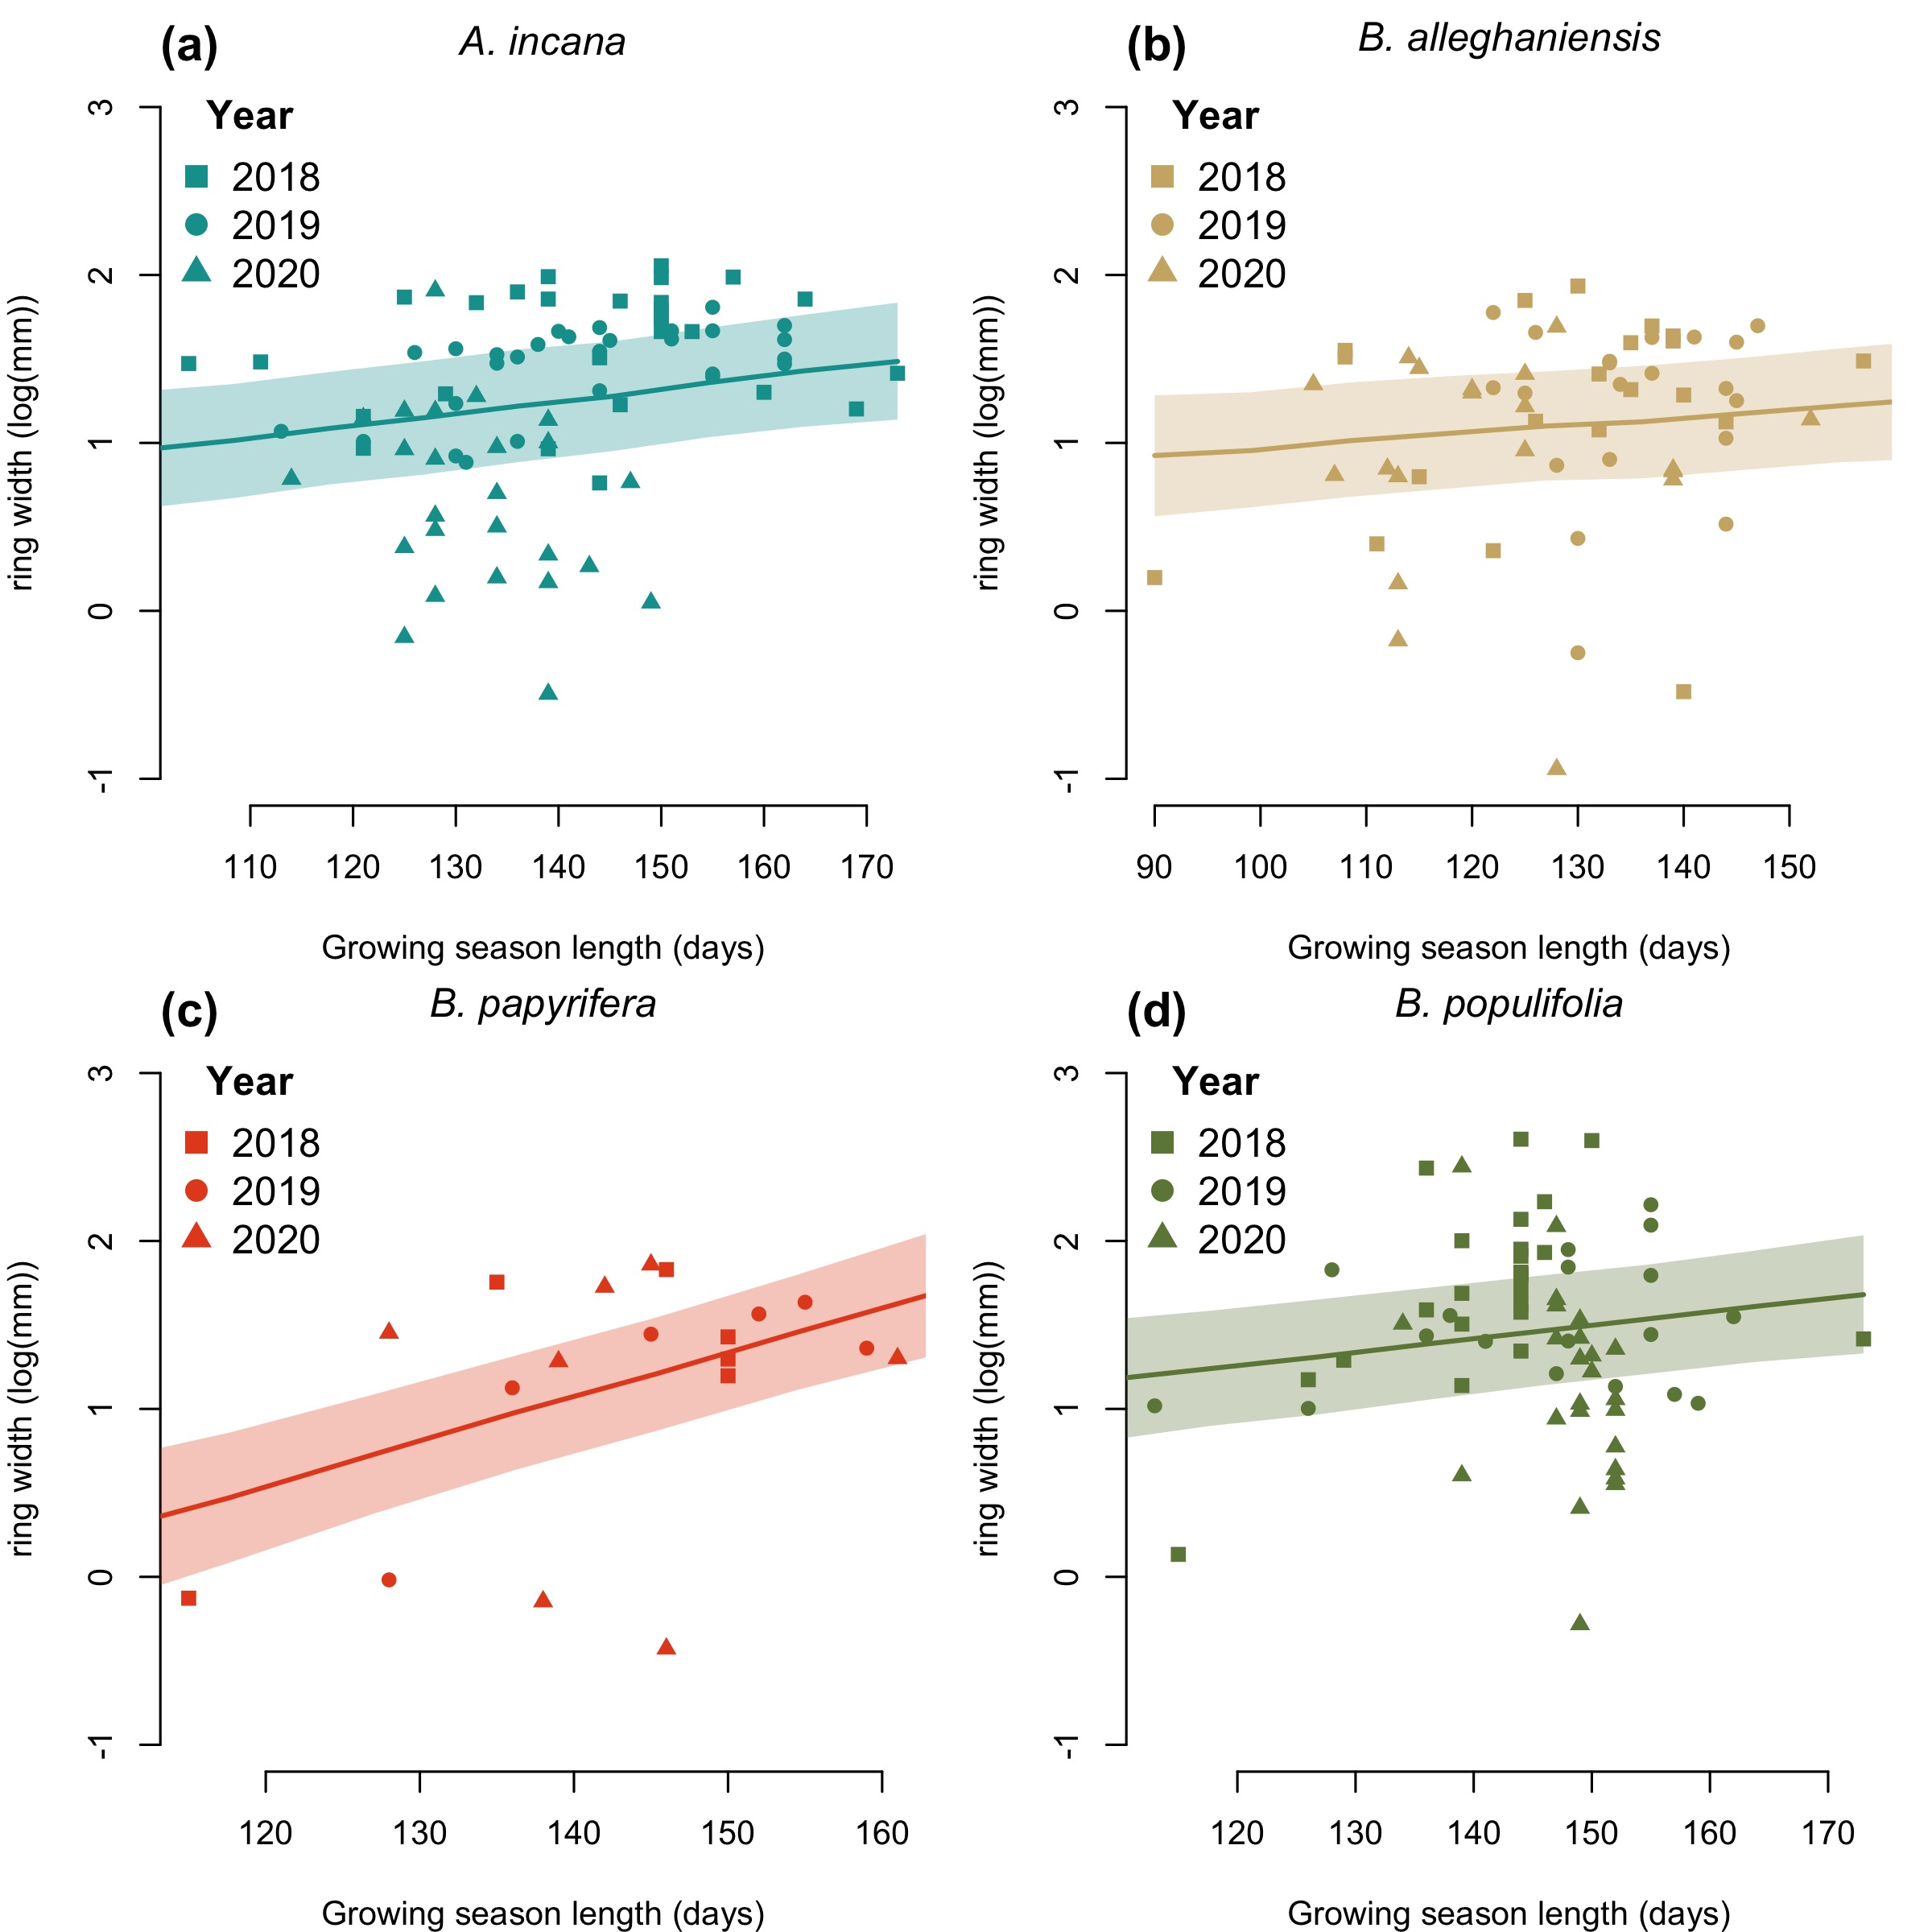
\includegraphics[width=0.8\textwidth]{../figures/wildchrokie/growthModelsMain/growthModelSlopesperSppFacetGSL.jpeg}
\caption{Ring width trends (log(mm)) in response to calendar season (growing season length). The plots are the reconstructed species estimates posterior distribution with error. The lines represent the mean of the posterior distribution and the shaded area, the 50\% UI at each predictor value. The dots are the empirical data shaped by year.}
\label{fig:wcxyGSL}
\end{figure}

% Figure mu atreeid full
\begin{figure}[!ht]
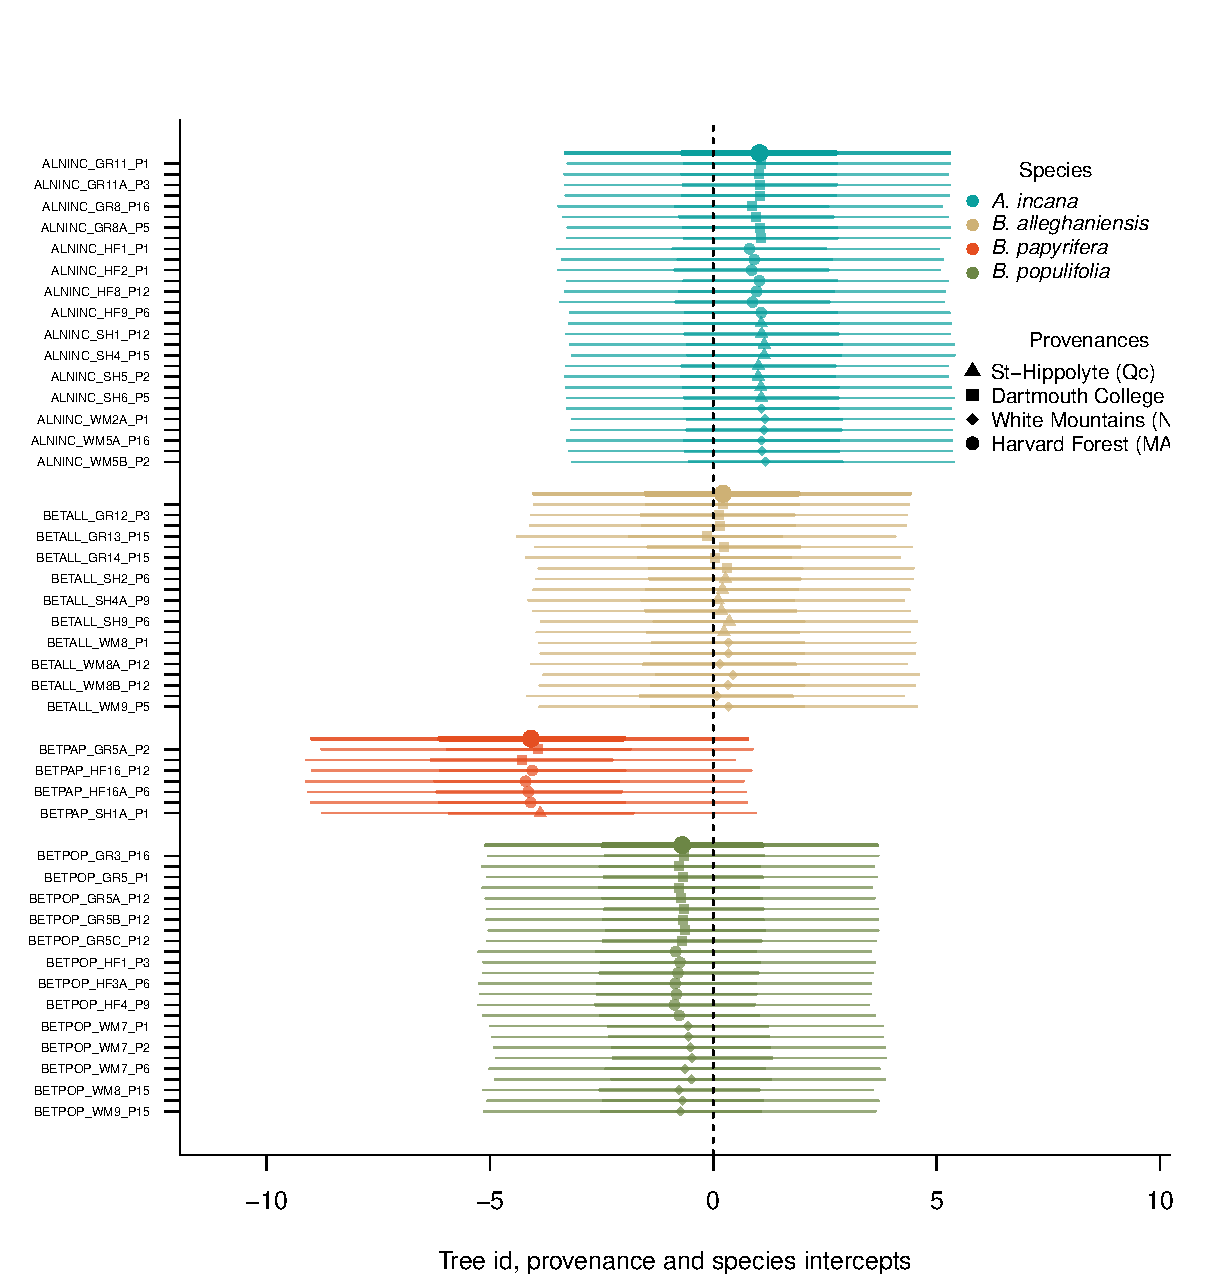
\includegraphics[width=0.8\textwidth]{../figures/wildchrokie/growthModelsMain/meanPlotGrowthGDD_treeidBYspp.pdf}
\caption{Ring width (log(mm)) deviations from the grand mean for grouping factor of the GDD model. The different tree id values represent the combined intercepts of tree id, provenance, species and averaged year intercepts. The larger dots and lines represent the species intercepts which are the species level estimates averaged across all of their tree ids. The dots are the mean of the posterior distribution and the thick and thin lines, the 50 and 90\% UI.}
\label{fig:wcmuplotatreeid}
\end{figure}

% Wildchrokie boxplot
\begin{figure}[!ht]

\includegraphics[width=1\textwidth]{../figures/wildchrokie/growthModelsMain/boxplotRingWidth.jpeg}
\caption{Boxplots representing the empirical data of our ring widths (mm) separated by species. The dots represent the raw data, the line is the mean and the box depicts the 50\% UI.}
\label{fig:wcboxplotRW}
\end{figure}

% Wildchrokie boxplot
\begin{figure}[!ht]

\includegraphics[width=1\textwidth]{../figures/wildchrokie/growthModelsMain/boxplotPredictorsAll.pdf}  
\caption{Boxplots representing the empirical data of all our predictors clustered by species, and for each year. The dots represent the raw data, the line is the mean and the box depicts the 50\% UI.}
\label{fig:wcboxplotPred}
\end{figure}

% Z-scored slope results Wildchrokie
\begin{figure}[!ht]

\includegraphics[width=0.8\textwidth]{../figures/wildchrokie/growthModelsMain/zscored/muALLbsppZ.pdf}
\caption{Effect size of each predictor across our four species. We depict ring width (log(mm)) change per adjusted predictor ($z$-scored; see data analyses section for more details) for each species. We report estimates as mean and 90\% uncertainty intervals (in square brackets) across our four different predictors (growing degree days, growing season length, start of season and end of season).}
\label{fig:bsppZscored}
\end{figure}


% Climate data overlap
\begin{figure}[!ht]
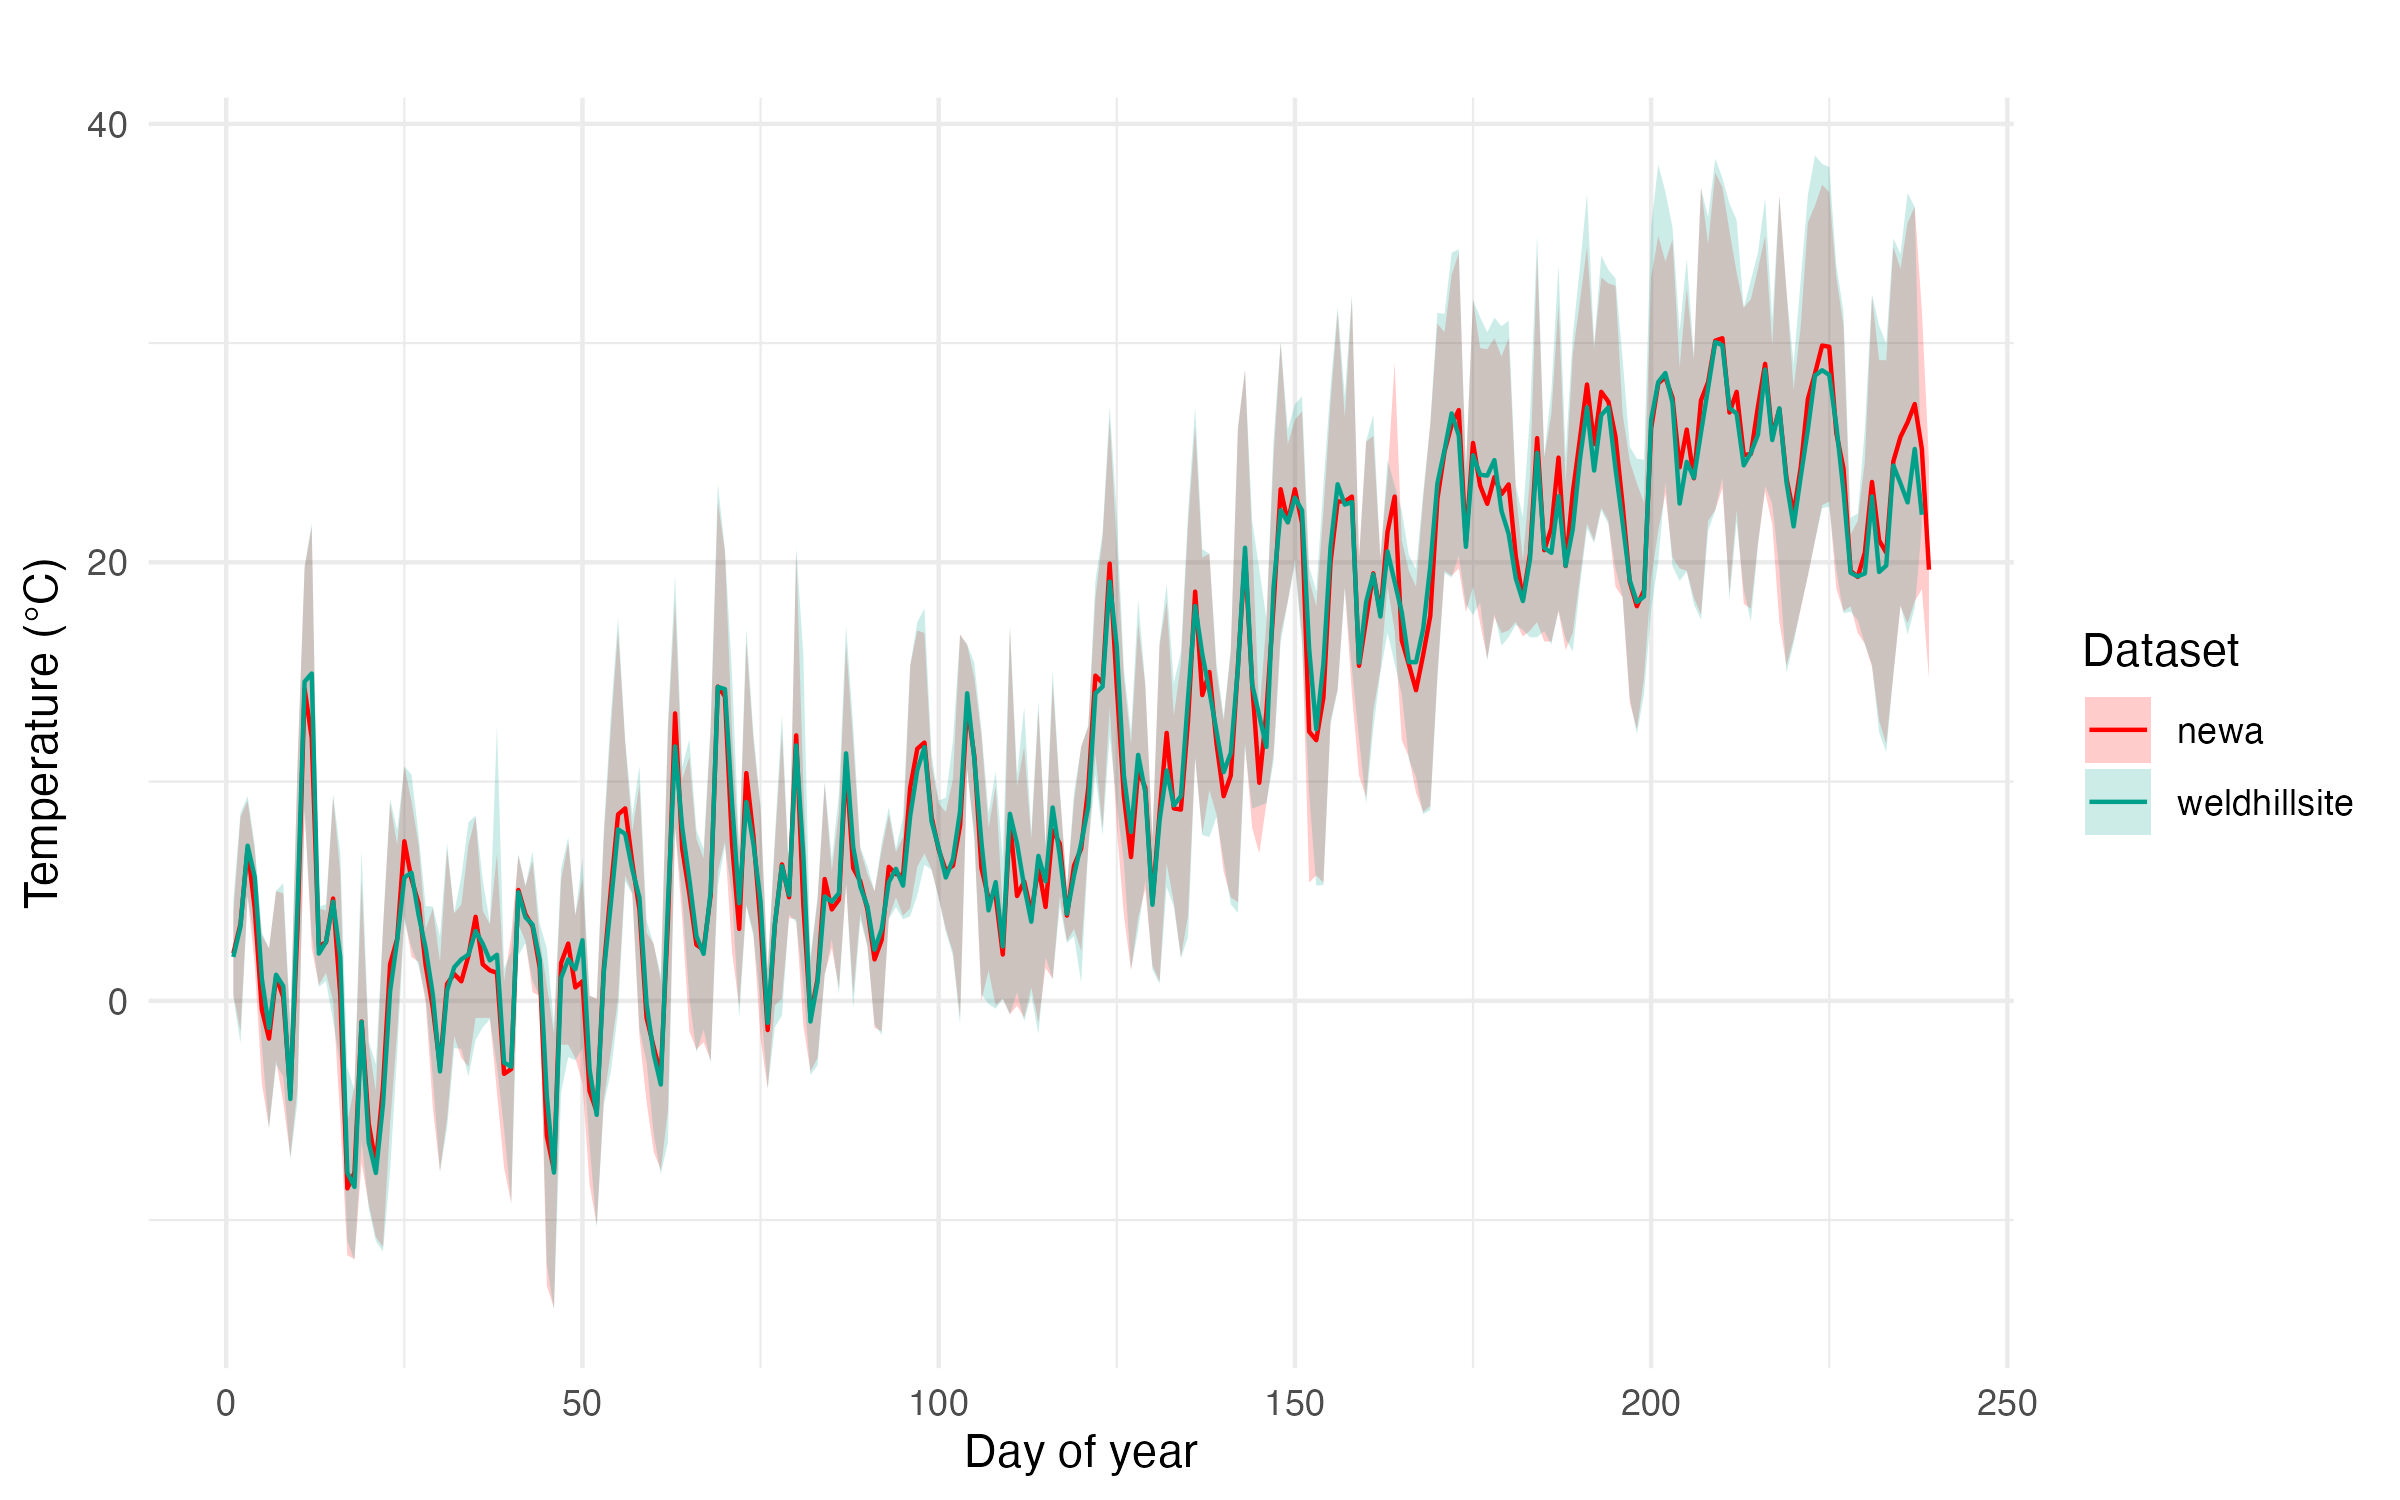
\includegraphics[width=0.7\textwidth]{../figures/climateComparison2020.jpeg}
\caption{Climate data overlap in 2020 for the two climate stations we used in our dataset (see data analyses section for more details). The lines represent the daily mean temperature of each climate station and the shaded area, the minimum and maximum daily temperature.}
\label{fig:climOverlap}
\end{figure}




